\documentclass{beamer}

\usepackage{amsmath}
\usepackage{graphicx}

\title{Introduction to Data Mining}
\author{Scott Powers and Ryan Wang}

\begin{document}

\begin{frame}
\titlepage
\end{frame}

\begin{frame}
\frametitle{RMS Titanic}
\begin{center}
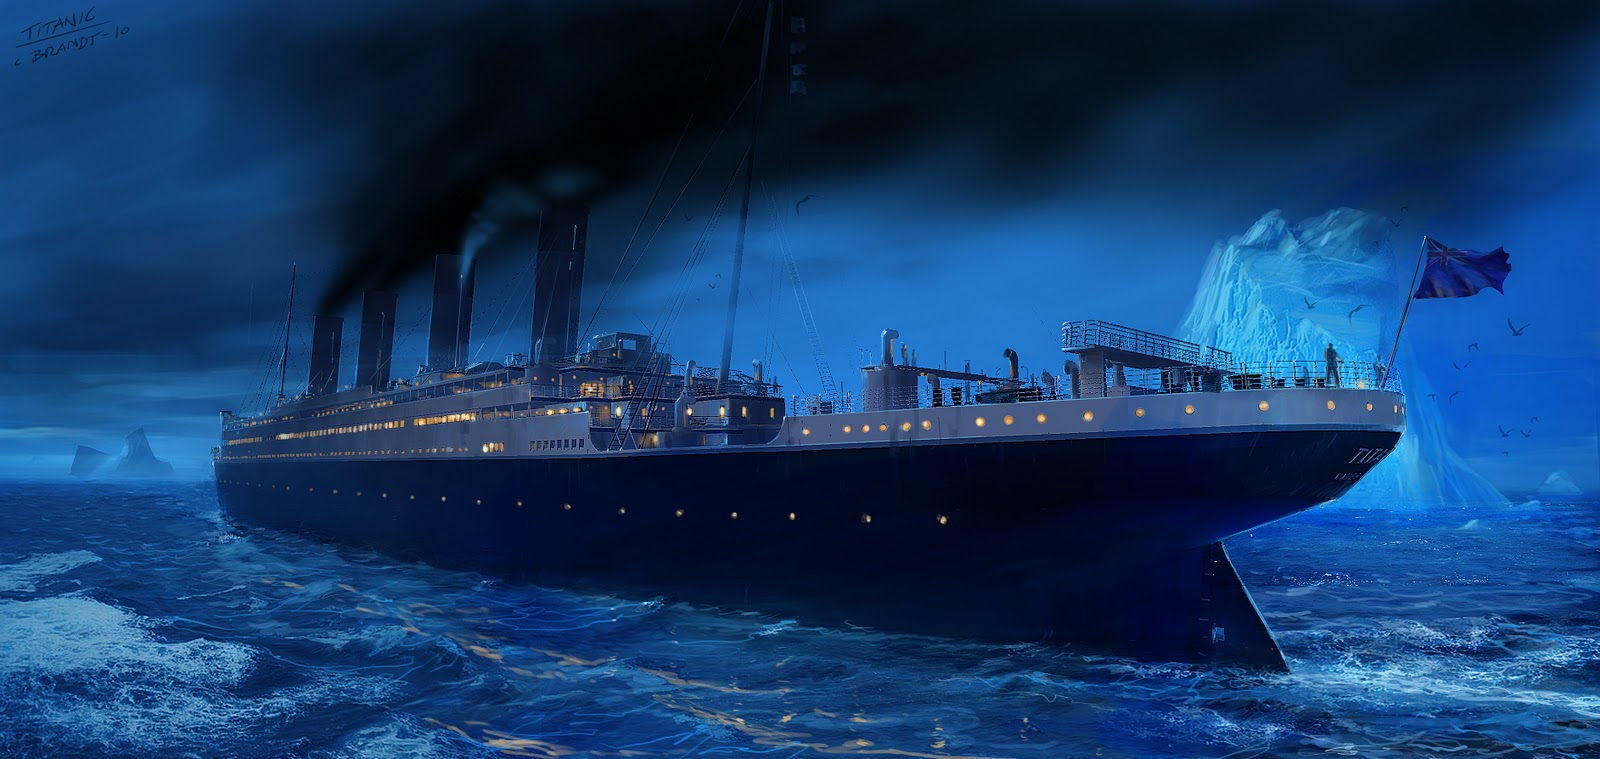
\includegraphics[scale = .15]{titanic.jpg}
\end{center}
\begin{itemize}
\item In 1912, the Titanic sank after colliding with an iceberg
\item Total number of passengers and crew: 2224
\begin{itemize}
\item How many people survived? \pause 722
\end{itemize}
\item Kaggle: Can we predict which passengers survived?
\end{itemize}
\end{frame}

\begin{frame}
\frametitle{The Data}
train.csv:
\begin{center}
{\tiny
\begin{tabular}{|r|r|r|l|r|r|r|r|r|r|r|r|}\hline
ID	& Su	& C	& Name				& S	& Age	& Sib/Sp	& Par/Ch	& Fare	& Cabin	& Port	\\\hline
1	& 0	& 3	& Braund, Owen		& M	& 22		& 1		& 0		& 7.25	& 		& S		\\\hline
2	& 1	& 1	& Cumings, Florence	& F	& 38		& 1		& 0		& 71.28	& C85	& C		\\\hline
3	& 1	& 3	& Heikkinen, Laina		& F	& 26		& 0		& 0		& 7.93	&		& S		\\\hline
4	& 1	& 1	& Futrelle, Lily			& F	& 35		& 1		& 0		& 53.10	& C123	& S		\\\hline
5	& 0	& 3	& Allen, William		& M	& 35		& 0		& 0		& 8.05	&		& S		\\\hline
6	& 0	& 3	& Moran, James		& M	& NA		& 0		& 0		& 8.46	&		& Q		\\\hline
...	& ...	& ...	& ...					& ...	& ...		& ...		& ...		& ...		& ...		& ...		\\\hline
891	& 0	& 3	& Dooley, Patrick		& M	& 32		& 0		& 0		& 7.75	&		& Q		\\\hline
\end{tabular}
}
\end{center}
test.csv:
\begin{center}
{\tiny
\begin{tabular}{|r|r|r|l|r|r|r|r|r|r|r|r|}\hline
ID	& Su	& C	& Name				& S	& Age	& Sib/Sp	& Par/Ch	& Fare	& Cabin	& Port	\\\hline
892	& ?	& 3	& Kelly, James			& M	& 35		& 0		& 0		& 7.83	& 		& Q		\\\hline
893	& ?	& 3	& Wilkes, Ellen			& F	& 47		& 1		& 0		& 7.00	&		& S		\\\hline
894	& ?	& 2	& Myles, Thomas		& M	& 62		& 0		& 0		& 9.69	&		& Q		\\\hline
...	& ...	& ...	& ...					& ...	& ...		& ...		& ...		& ...		& ...		& ...		\\\hline
1309	& ?	& 3	& Peter, Michael		& M	& NA		& 1		& 1		& 22.36	&		& C		\\\hline
\end{tabular}
}
\end{center}
Brainstorm: What kind of person is more likely to survive?
\end{frame}

\end{document}